\documentclass[a4paper, 11pt]{book}
\usepackage{/home/nicolas/Documents/Enseignement/Prepa/bpep/fichiers_utiles/preambule}

\raggedbottom

\newcommand{\dsNB}{14}
\makeatletter
\renewcommand{\@chapapp}{Kh\^olles MPSI3 -- semaine \dsNB}
\makeatother

\toggletrue{corrige}  % décommenter pour passer en mode corrigé

 % IMPORTS automatiques
\newcommand{\f}[2]{{
		\mathchoice
		{\dfrac{#1}{#2}}
		{\dfrac{#1}{#2}}
		{\frac{#1}{#2}}
		{\frac{#1}{#2}}
}}

\newcommand{\e}[1]{{}_{\text{#1}}}

 % fin des IMPORTS automatiques

\begin{document}

\chapter{Sujet 1\siCorrige{\!\!-- corrig\'e}}
\section{Question de cours}

Présenter ce qu'est une onde progressive sinusoïdale, établir sa
        double périodicité, indiquer les différentes relations reliant $\omega$
        et $f$ ou $T$~; $k$ et $\lambda$~; $\lambda$, $c$ et $f$ ou $T$. Définir
        un milieu dispersif et donner des exemples.

\resetQ
\subimport{/home/nicolas/Documents/Enseignement/Prepa/bpep/exercices/Colle/onde_progressive_transmission/}{sujet.tex}


\chapter{Sujet 2\siCorrige{\!\!-- corrig\'e}}
\section{Question de cours}
On considère ici un mascaret qui se déplace à la vitesse $c =
\SI{18}{km.h^{-1}}$ le long d'un fleuve rectiligne, et on définit un axe
$(Ox)$ dans la direction du sens de sa propagation.

À l'instant $t=0$, le profil du niveau de l'eau du fleuve a l'allure
suivante~:
\begin{center}
    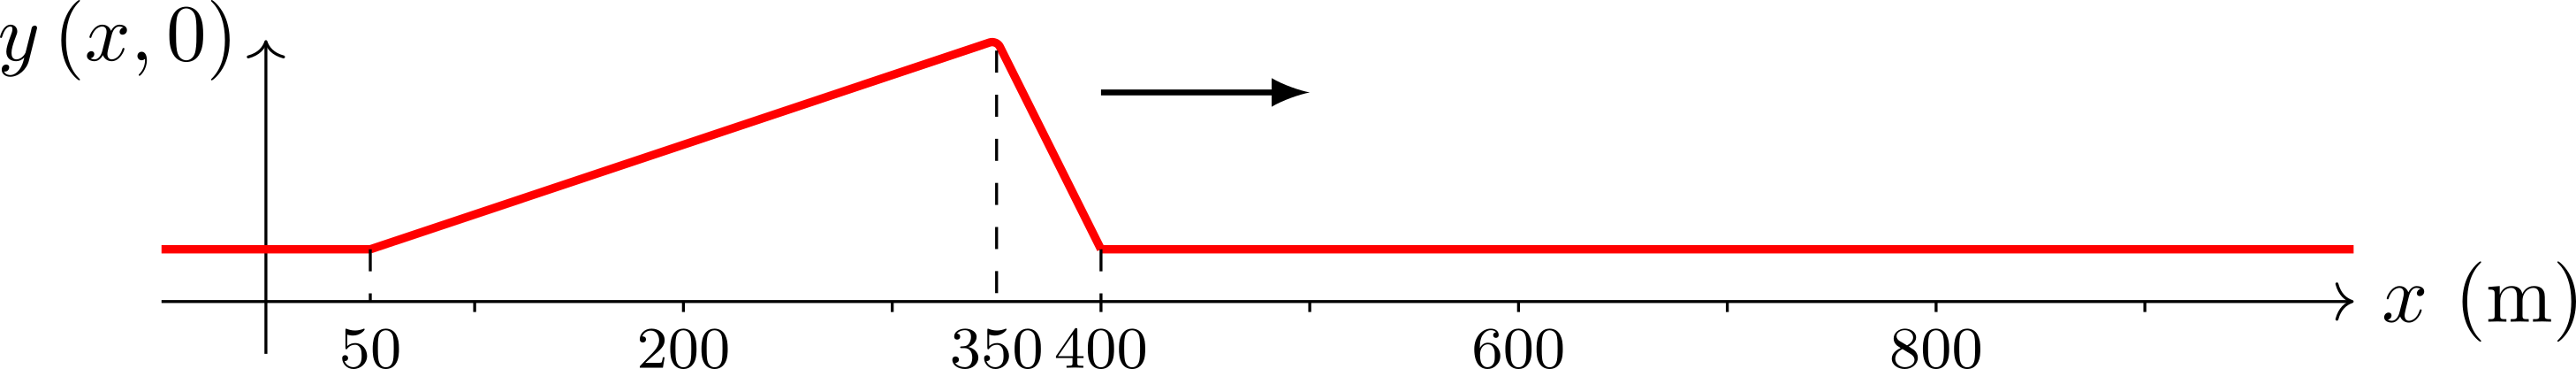
\includegraphics[width=0.8\linewidth]{../../figures/ch14/rep_spa-masc_a}
\end{center}
\begin{enumerate}[label=\sqenumi]
    \item Faire un schéma du profil du fleuve à $\tau = \SI{1}{min}$ en
        supposant que l'onde se propage sans déformation.
    \item À quel instant la vague arrive-t-elle au point d'abscisse $x_1 =
        \SI{2.2}{km}$~? 
    \item Un détecteur fixe, enregistrant la hauteur du fleuve en fonction
        du temps, est placé à l'abscisse $x_d = \SI{1.6}{km}$. Dessiner
        l'allure des variations $y(x_d,t)$ en fonction du temps à cette
        abscisse.
\end{enumerate}

\resetQ
\subimport{/home/nicolas/Documents/Enseignement/Prepa/bpep/exercices/Colle/onde_sismique/}{sujet.tex}

\chapter{Sujet 3\siCorrige{\!\!-- corrig\'e}}
\section{Question de cours}
Déterminer l'expression du signal somme de deux ondes sinusoïdales de
même fréquence \textbf{et même amplitude} en introduisant $\Delta
\varphi(\Mr)$ et $\varphi_0(\Mr)$. Définir et déterminer son intensité lumineuse.
On la mettra sous la forme de la formule de \textsc{Fresnel}. Exprimer
les valeurs de $\Delta\varphi(\Mr)$ correspondant à des interférences
constructives ou destructives.

\resetQ
\subimport{/home/nicolas/Documents/Enseignement/Prepa/bpep/exercices/Colle/onde_progressive/}{sujet.tex}

\resetQ
\subimport{/home/nicolas/Documents/Enseignement/Prepa/bpep/exercices/TD/telemetre/}{sujet.tex}


\label{LastPage}

\end{document}
